
%This is a Tex Version of NE 806 Homework Template
%
\documentclass{amsart}
\setlength{\textheight}{9in}
\setlength{\topmargin}{-0.25in}
\setlength{\textwidth}{7in}
\setlength{\evensidemargin}{-0.25in}
\setlength{\oddsidemargin}{-0.25in}
\usepackage{amsfonts}
\usepackage[utf8]{inputenc}
\usepackage[T1]{fontenc}
\usepackage{graphicx} 
\usepackage[export]{adjustbox}
% needed to include these graphics
%\graphicspath{{./Pictures/}}      % only in case you want to keep the pictures in a separate
                                  % subdirectory; also see the appropriate line below
\usepackage{caption}
\usepackage{subcaption}
\usepackage{float}
\usepackage{framed}
\newcounter{temp}
\theoremstyle{definition}
\newtheorem{Thm}{Theorem}
\newtheorem{Prob}{Problem}
\newtheorem*{Def}{Definition}
\newtheorem*{Ans}{Answer}
\newcommand{\dis}{\displaystyle}
\newcommand{\dlim}{\dis\lim}
\newcommand{\dsum}{\dis\sum}
\newcommand{\dint}{\dis\int}
\newcommand{\ddint}{\dint\!\!\dint}
\newcommand{\dddint}{\dint\!\!\dint\!\!\dint}
\newcommand{\dt}{\text{d}t}
\newcommand{\dA}{\text{d}A}
\newcommand{\dV}{\text{d}V}
\newcommand{\dx}{\text{d}x}
\newcommand{\dy}{\text{d}y}
\newcommand{\dz}{\text{d}z}
\newcommand{\dw}{\text{d}w}
\newcommand{\du}{\text{d}u}
\newcommand{\dv}{\text{d}v}
\newcommand{\ds}{\text{d}s}
\newcommand{\dr}{\text{d}r}
\newcommand{\dth}{\text{d}\theta}
\newcommand{\bbR}{\mathbb{R}}
\newcommand{\bbN}{\mathbb{N}}
\newcommand{\bbQ}{\mathbb{Q}}
\newcommand{\bbZ}{\mathbb{Z}}
\newcommand{\bbC}{\mathbb{C}}
\newcommand{\dd}[2]{\dfrac{\text{d}#1}{\text{d}#2}}
\newcommand{\dydx}{\dfrac{\text{d}y}{\text{d}x}}
\renewcommand{\labelenumi}{{\normalfont \arabic{enumi}.}}
\renewcommand{\labelenumii}{{\normalfont \alph{enumii}.}}
\renewcommand{\labelenumiii}{{\normalfont \roman{enumiii}.}}
\font \bggbf cmbx18 scaled \magstep2
\font \bgbf cmbx10 scaled \magstep2
\usepackage{fancyhdr}
\usepackage{lipsum}
% Clear the header and footer
\fancyhead{}
\fancyfoot{}
% Set the right side of the footer to be the page number
\rfoot{\thepage}
\fancyhf{}
\pagestyle{fancy}
\begin{document}
\LARGE{NE-806: Neutronics}
 
\large
Homework \#3 due Thurs. October 23, 2018
 
Solutions by: John Boyington

Note: Code used in this assignment is all located at https://github.com/johnboyington/ne806/tree/master/hw3 and available for download/use.
\bigskip
 

%%%%%%%%%%%%%%%%%%%%%%%%%%%%%%%%%%%%%%%%%%%%%%%%%%%%%%%%%%%%%%%%%%%%%%%%%%%%%%%%%%%%%%%%%%%%%%%%%%%%%%%%%%%%%%%%%%%%%%%%%%%
%                                        PROBLEM 1
%%%%%%%%%%%%%%%%%%%%%%%%%%%%%%%%%%%%%%%%%%%%%%%%%%%%%%%%%%%%%%%%%%%%%%%%%%%%%%%%%%%%%%%%%%%%%%%%%%%%%%%%%%%%%%%%%%%%%%%%%%%
\textbf{Problem 1:} Consider a homogeneous infinite slab of thickness $2T$ located in a vacuum. Write a
Monte Carlo program to calculate (a) $k_{eff}$, (b) the neutron leakage probability $PL$, and (c) the critical flux density distribution. Assume that a one-speed transport model can be used and that scattering and fission neutrons are emitted isotropically in the laboratory coordinate system.
\bigbreak
Your code should include the following features:
\bigbreak
(a) the use of multiple batches (or games) so as to permit an estimate of the standard deviation of the final result for $k_{eff}$ and $PL$\newline
\bigbreak
(b) the use of a spatially uniform source distribution for the first game, and then, for later games, a source that is adaptively distributed according to the fission distribution\newline
\bigbreak
(c) accumulation of the spatial distribution of fission events from game to game (after the first few games) so as to obtain an increasingly better estimate of the fission source distribution (as well as the critical flux density profile)\newline
\bigbreak
Use your Monte Carlo code to obtain data to create a plot of $k_{eff}$ versus slab thickness $2T$ over the range from 30 to 80 cm for a slab material with the following nuclear properties:
\bigbreak
\begin{equation*}
    \Sigma_c = 0.011437\quad cm^{-1}, \quad \Sigma_s = 0.05\quad cm^{-1}, \quad \Sigma_f = 0.013\quad cm^{-1}, \quad \nu=2.5
\end{equation*}
\bigbreak
Of particular interest is the thickness $2T = 53.744$ cm. Find the critical thickness for this slab and plot the critical flux profile.
\bigbreak
%%%%%%%%%%%%%%%%%%%%%%%%%%%%%%%%%%%%%%%%%%%%%%%%%%%%%%%%%%%%%%%%%%%%%%%%%%%%%%%%%%%%%%%%%%%%%%%%%%%%%%%%%%%%%%%%%%%%%%%%%%%
\textbf{Solution}

Using my Monte Carlo code, I was able to create the following plot that shows the $k_{eff}$ against half thickness $T$.
Shown also is the flux profile for the thickness $2T = 53.744$ cm.
The flux profile shows how it is updated over time, with the darkest lines being the most current batches.
These were run with 15 batches and a batch size of $1 \times 10^6$ histories.

\begin{center}
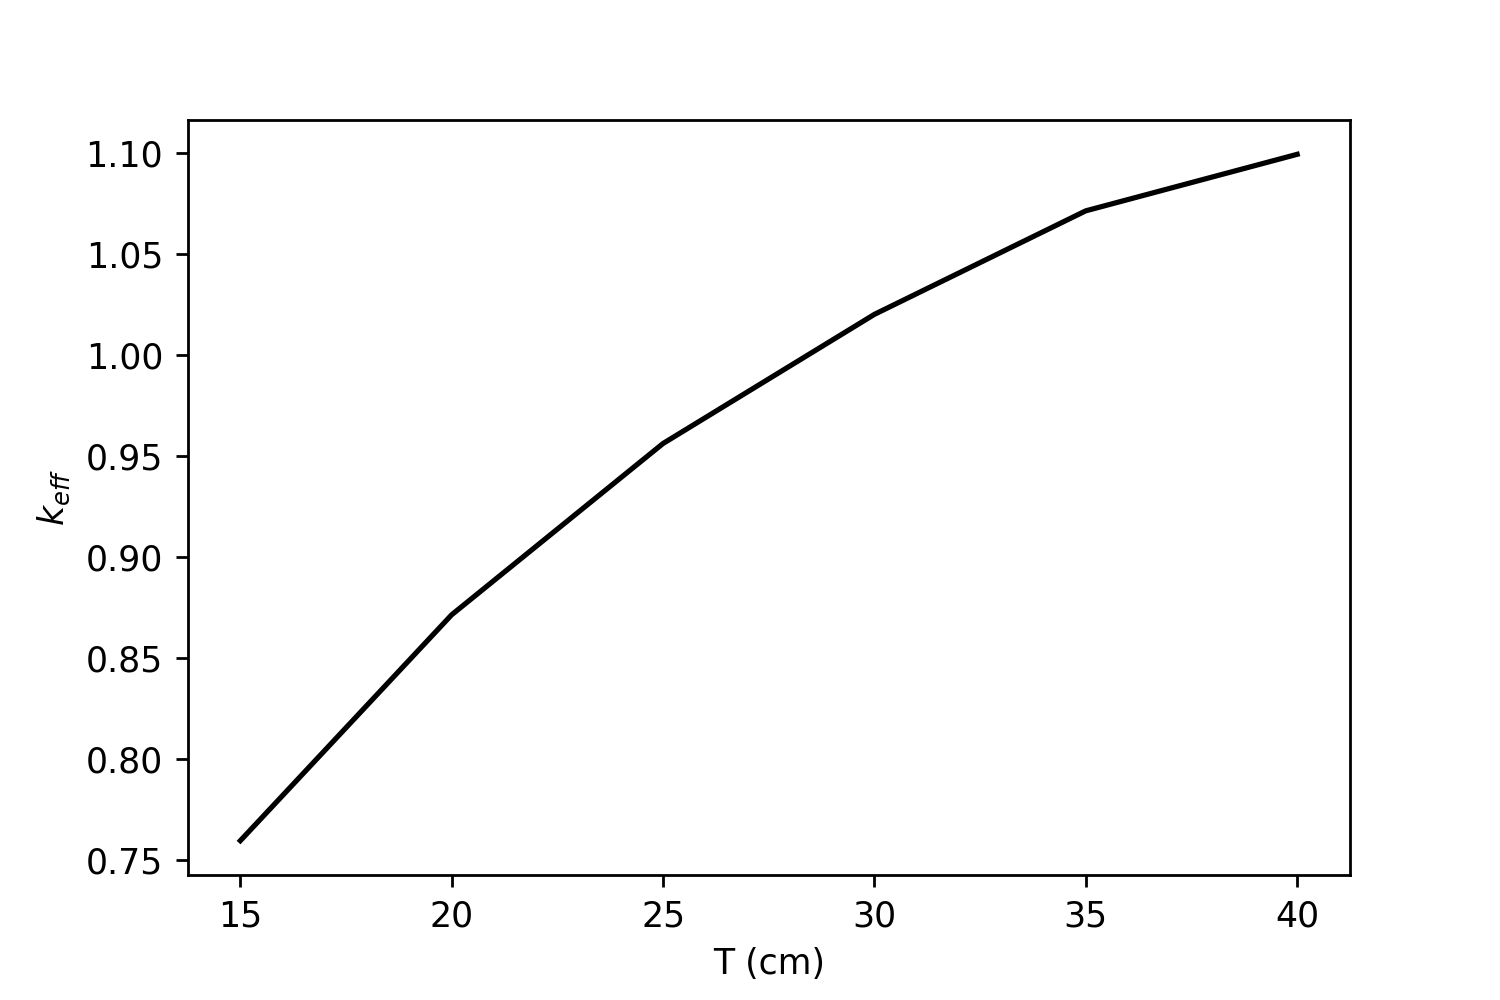
\includegraphics[totalheight=.40\textheight]{k_vs_T.png}
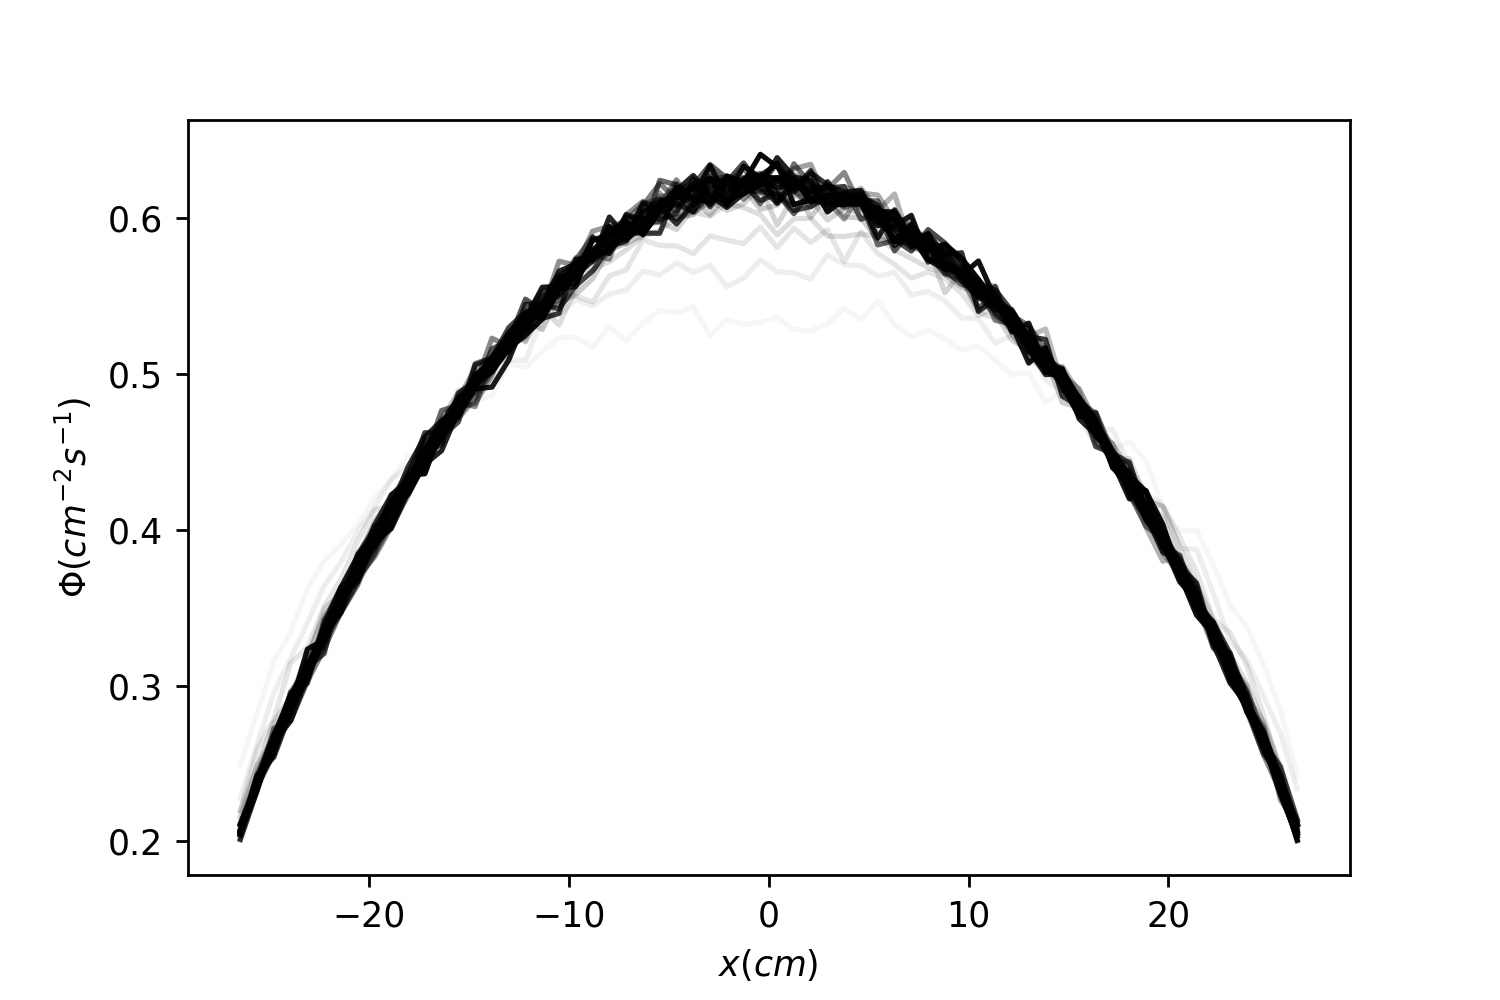
\includegraphics[totalheight=.40\textheight]{t_crit.png}
\end{center}

The $k_eff$ increases with increasing $T$.
This follows intuition, which suggests that as more material is available for reflection and fissioning, the more neutrons will remain non-leaked.

The code, as written, currently contains a full implementation of the algorithm described in the lecture 13 slides.
It begins with a flat profile for the fission, and then as it tallies $N_f$, the number of fissions in a particular spatial region, it replaces the source sampling with the latest fission distribution.
Particles are ran in batches, each particle is born with a particular position and direction.
From there, a distance is selected for the particle to travel using $\Sigma_t$.
If the particle leaks or absorbed, a new history is began.
If it scatters, then a new direction and travel distance is chosen.


 
%%%%%%%%%%%%%%%%%%%%%%%%%%%%%%%%%%%%%%%%%%%%%%%%%%%%%%%%%%%%%%%%%%%%%%%%%%%%%%%%%%%%%%%%%%%%%%%%%%%%%%%%%%%%%%%%%%%%%%%%%%%
%                                        PROBLEM 2
%%%%%%%%%%%%%%%%%%%%%%%%%%%%%%%%%%%%%%%%%%%%%%%%%%%%%%%%%%%%%%%%%%%%%%%%%%%%%%%%%%%%%%%%%%%%%%%%%%%%%%%%%%%%%%%%%%%%%%%%%%%
\newpage
\textbf{Problem 2:}Write anther computer program to solve for the critical value of $c$, $c_{crit}$, using the one speed integral transport equation with isotropic fission and scattering, for an infinite bare homogeneous slab. With the results from your program, plot $ln (c_{crit} - 1)$ versus the slab thickness $2T$ for $0<2T<10$ mean-free-path lengths. HINT: as a check on your program, you should obtain $c_{crit}$ = 1.277101824 . . . when the thickness of the slab is 2 mean-free-path lengths.
\bigbreak
 
%%%%%%%%%%%%%%%%%%%%%%%%%%%%%%%%%%%%%%%%%%%%%%%%%%%%%%%%%%%%%%%%%%%%%%%%%%%%%%%%%%%%%%%%%%%%%%%%%%%%%%%%%%%%%%%%%%%%%%%%%%%
\textbf{Solution}

The code was implemented to solve the NTE and was ran for slab thicknesses between $0<T<5$ mean-free-path lengths.

\begin{center}
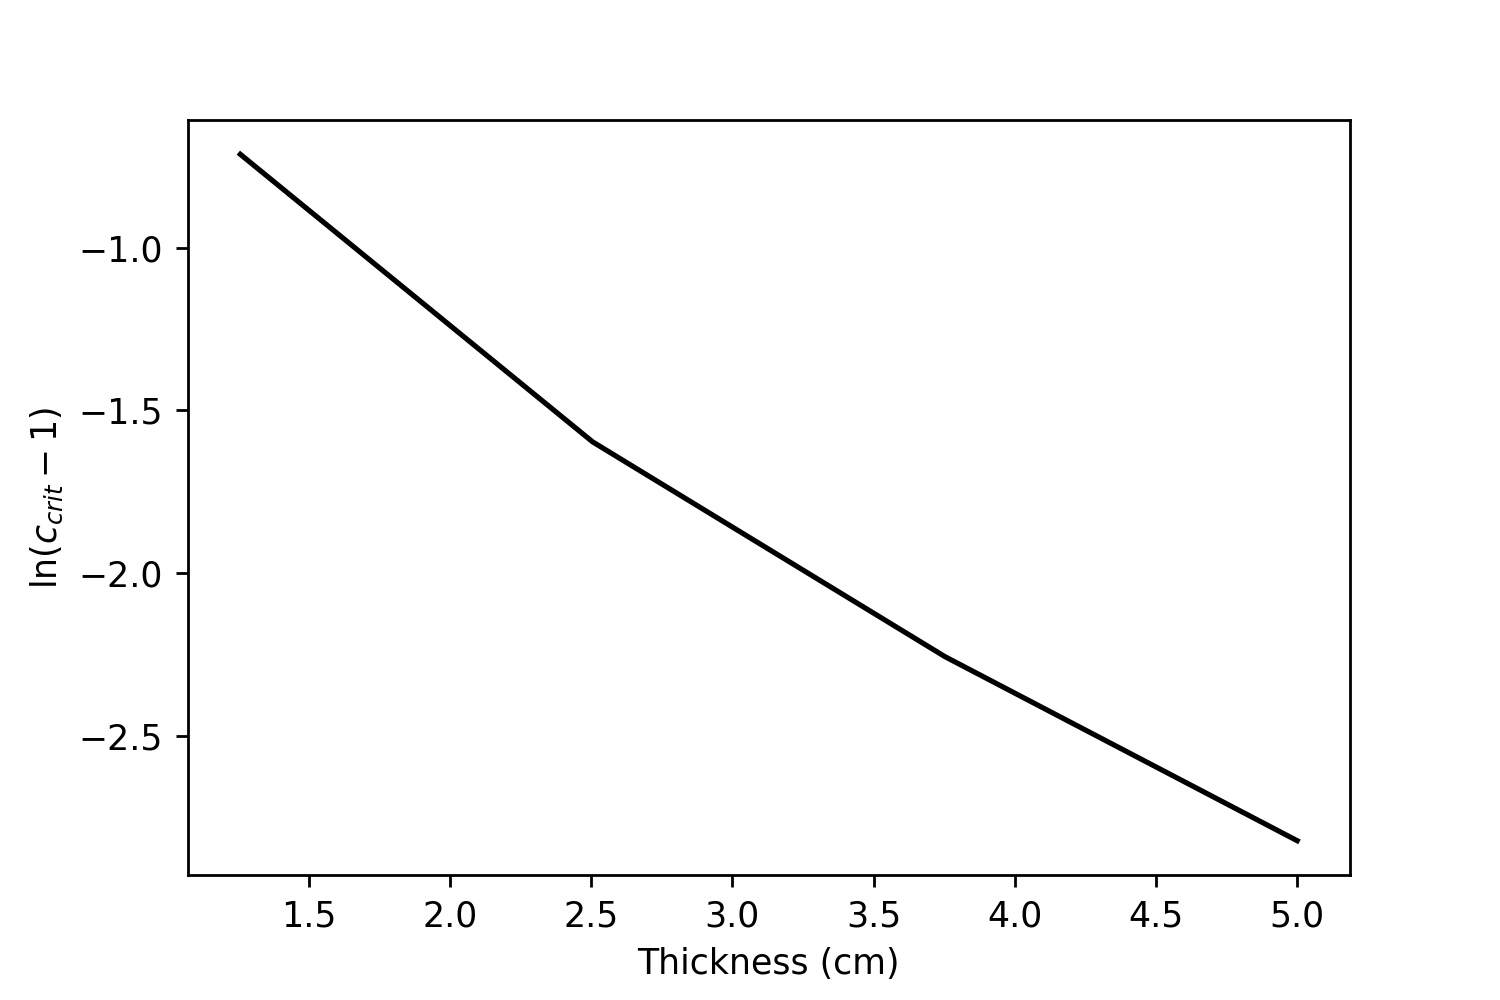
\includegraphics[totalheight=.40\textheight]{c_crit.png}
\end{center}

This code, using the procedures described in lecture 9, uses power iteration to solve the following represenation of the transport equation:

$$ B \Phi = \frac{2}{c} \Phi $$

First, the $B$ matrix is prepared, which represents the effect that a flux in any particular cell will have on each other cell.
Then the power iteration method, takes an initial $\Phi$, which in our case is an identity array, and iteratively updates $\Phi$ and $c$, until converging within some nominal tolerance.
 
%%%%%%%%%%%%%%%%%%%%%%%%%%%%%%%%%%%%%%%%%%%%%%%%%%%%%%%%%%%%%%%%%%%%%%%%%%%%%%%%%%%%%%%%%%%%%%%%%%%%%%%%%%%%%%%%%%%%%%%%%%%
%                                        PROBLEM 3
%%%%%%%%%%%%%%%%%%%%%%%%%%%%%%%%%%%%%%%%%%%%%%%%%%%%%%%%%%%%%%%%%%%%%%%%%%%%%%%%%%%%%%%%%%%%%%%%%%%%%%%%%%%%%%%%%%%%%%%%%%%
\newpage
\textbf{Problem 3:} Use your NTE code to find the critical thickness of the slab analyzed with the Monte Carlo method in your first problem set ($\Sigma_c = 0.011437\quad cm^{-1}, \quad \Sigma_s = 0.05\quad cm^{-1}, \quad \Sigma_f = 0.013\quad cm^{-1}, \quad \nu=2.5$).
Compare the critical flux profiles found by each method.
\bigbreak
%%%%%%%%%%%%%%%%%%%%%%%%%%%%%%%%%%%%%%%%%%%%%%%%%%%%%%%%%%%%%%%%%%%%%%%%%%%%%%%%%%%%%%%%%%%%%%%%%%%%%%%%%%%%%%%%%%%%%%%%%%%
\textbf{Solution}

Shown on the following graph is the comparison for a slab of thickness $2T = 53.744$ cm.

\begin{center}
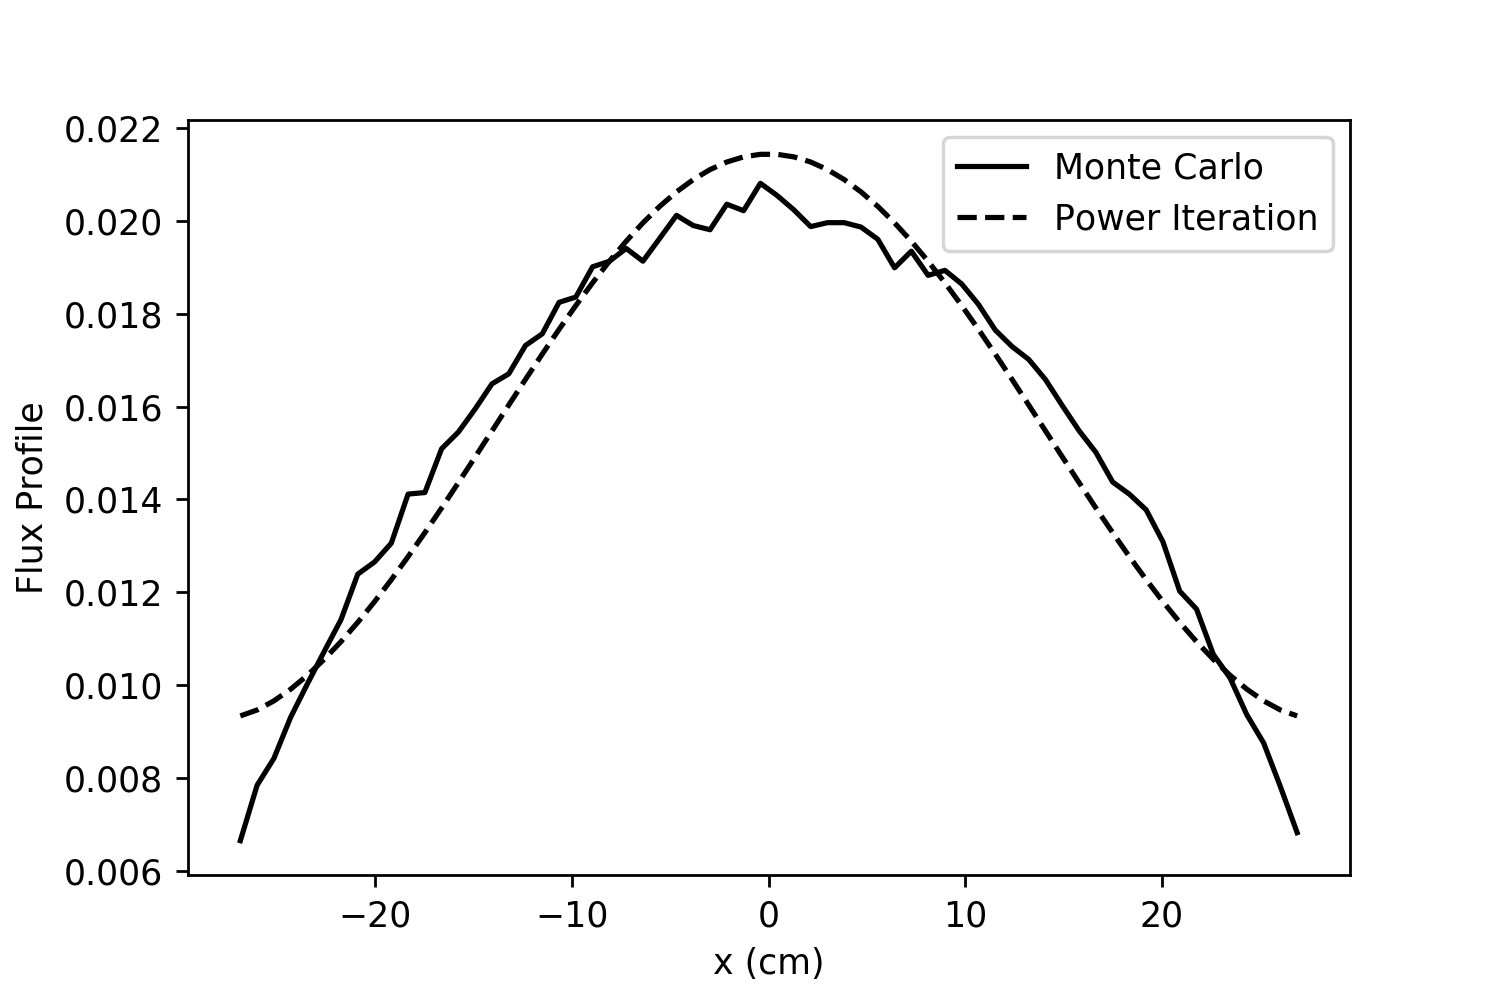
\includegraphics[totalheight=.40\textheight]{comparison.png}
\end{center}

The profiles have both been normalized to one - each is comprised of 64 bins.
The Monte Carlo solution is much more noisy, obviously a result of the stochastic nature of MC simulation.
However, the tail and inflection seen in power iteration is also not present within the MC results.
Instead, it curved downward across the entire domain.

%%%%%%%%%%%%%%%%%%%%%%%%%%%%%%%%%%%%%%%%%%%%%%%%%%%%%%%%%%%%%%%%%%%%%%%%%%%%%%%%%%%%%%%%%%%%%%%%%%%%%%%%%%%%%%%%%%%%%%%%%%%
%                                        PROBLEM 4
%%%%%%%%%%%%%%%%%%%%%%%%%%%%%%%%%%%%%%%%%%%%%%%%%%%%%%%%%%%%%%%%%%%%%%%%%%%%%%%%%%%%%%%%%%%%%%%%%%%%%%%%%%%%%%%%%%%%%%%%%%%
\newpage
\textbf{Problem 4:}Compare the critical flux profiles obtained with transport and diffusion theories for both a thin and thick slab (say, for example, T = 0.5 and T = 10 mean-free path lengths).
\bigbreak
Complete documentation of your programs, including theory, example outputs, and a detailed discussion of your results is required.
\bigbreak
%%%%%%%%%%%%%%%%%%%%%%%%%%%%%%%%%%%%%%%%%%%%%%%%%%%%%%%%%%%%%%%%%%%%%%%%%%%%%%%%%%%%%%%%%%%%%%%%%%%%%%%%%%%%%%%%%%%%%%%%%%%
\textbf{Solution}

The following two plots compare $T=0.5mfp$ (top) and $T=10mfp$ (bottom).
It can be seen that the diffusion approximation, while performing better for the larger case, performs terribly in the 0.5 mfp case.
This is due in part to the diffusion approximation's dealing with boundary conditions.
For the shorter case, the extrapolated boundary is well beyond the edges of the domain of the problem.
Because the diffusion approximation is simply a functional fit, it cannot capture these effects properly in a small region.
Transport theory is much more applicable to either case, and more properly captures the flux through the medium.

\begin{center}
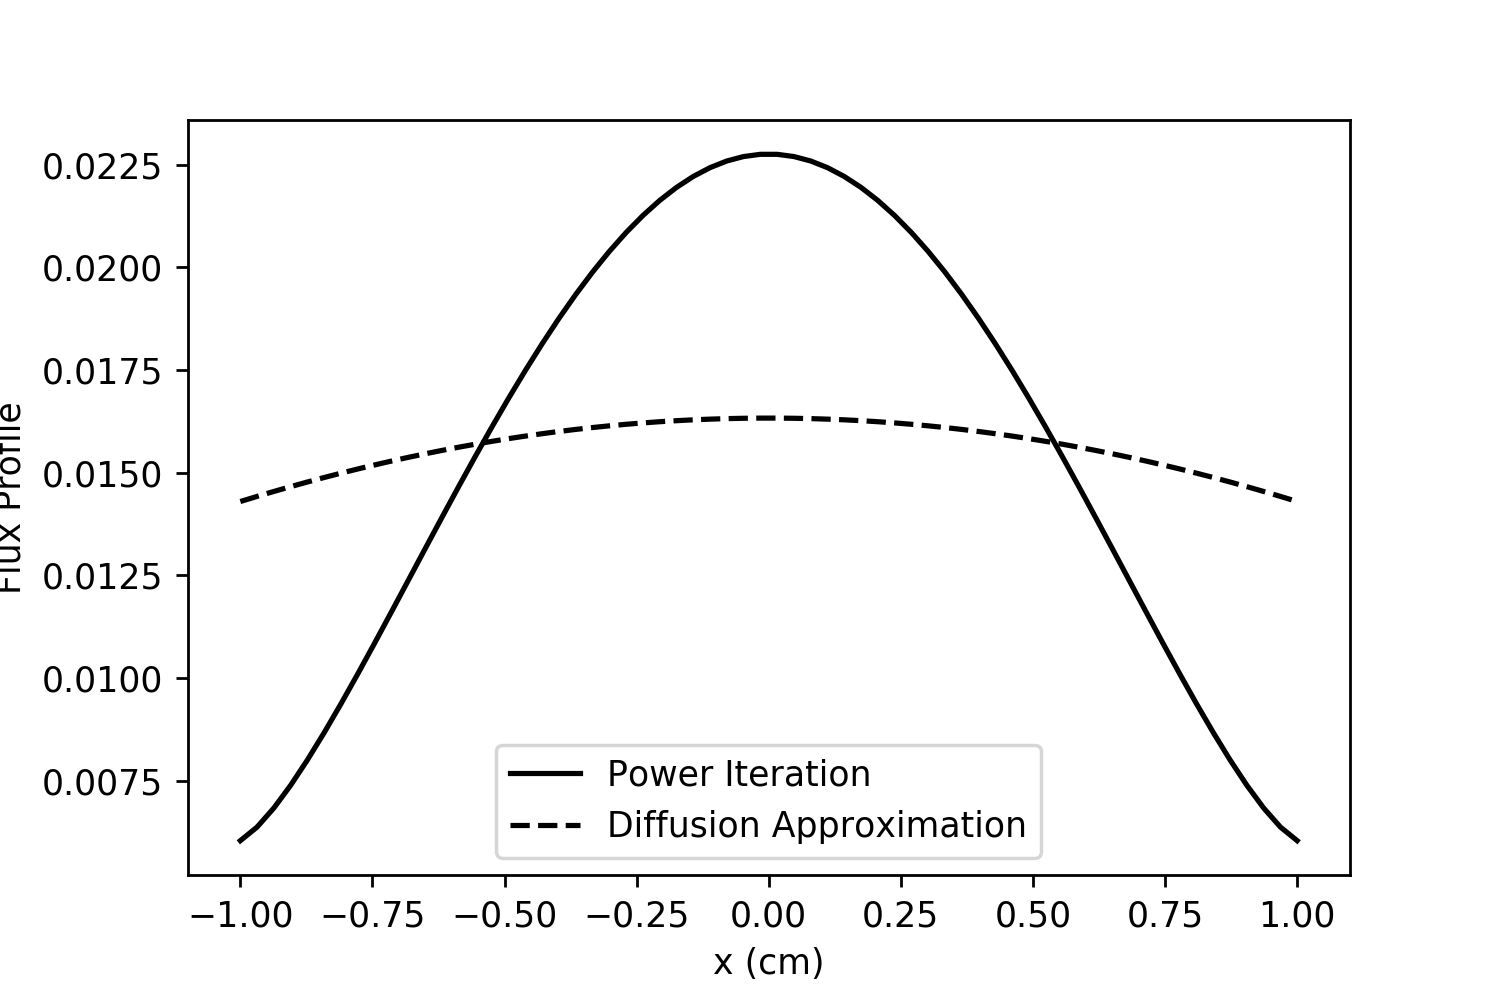
\includegraphics[totalheight=.40\textheight]{p4_05.png}
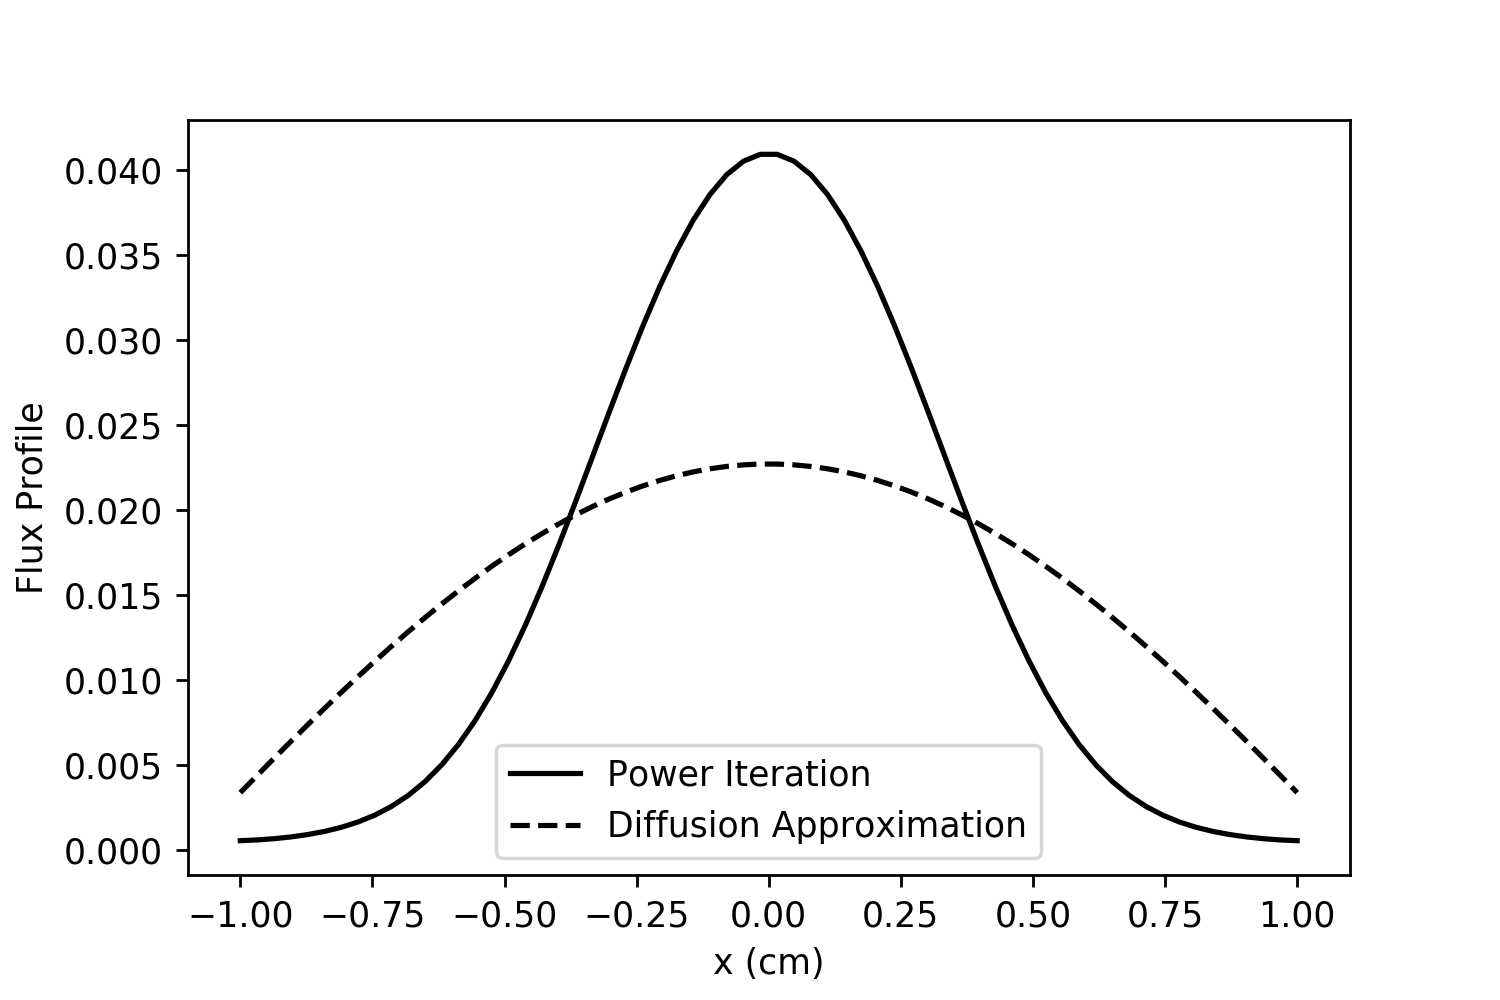
\includegraphics[totalheight=.40\textheight]{p4_10.png}
\end{center}


 
%%%%%%%%%%%%%%%%%%%%%%%%%%%%%%%%%%%%%%%%%%%%%%%%%%%%%%%%%%%%%%%%%%%%%%%%%%%%%%%%%%%%%%%%%%%%%%%%%%%%%%%%%%%%%%%%%%%%%%%%%%%
\end{document}

